In this section, we'll discuss some experiments that we have performed with the two different models. These experiments aimed to see which hyperparameters have significant effects on how well the models train. The models will primarily be evaluated based on how good their representation of the proteins is. To this end, we use the stability dataset described earlier. For each model, we then train a simple linear regression model on the model's representation of the proteins, against the given stability scores. How well this does is measured using spearman's rho.
\subsection{LSTM}  % casper
%\subsubsection{Embeddings vs no embeddings} % Consider deleting if lacking time
%Embedding is a good way to encode the differences and similarities between tokens. In the case of proteins, there are some amino acids that can potentially replace others with no effect on the resulting structure of the protein. Thus, being able to learn that some amino acids are very similar is a potentially helpful tool for next token prediction. For this experiment we've trained two models with the following identical hyperparameters:
\begin{itemize}
	\item Layers: $1$
	\item Starting learning rate: $8e-4$
	\item Learning rate schedule: Multiply by $0.2$ every 5 epochs
	\item Hidden layer size: $512$
	\item Training time: 30 epochs
\end{itemize}
The only difference between the two models is that one is trained on a onehot representation of the amino acids, while the other also learns a 30-dimensional embedding.\\

\noindent
Since embeddings will likely show some crucial similarities and differences between individual amino acids, we hypothesise that embeddings will significantly increase the performance of the network.

\subsubsection{Layers vs no layers} % Finished
\begin{figure}[h]
	% Accuracy on test set: 12.43%, loss 2.84
  	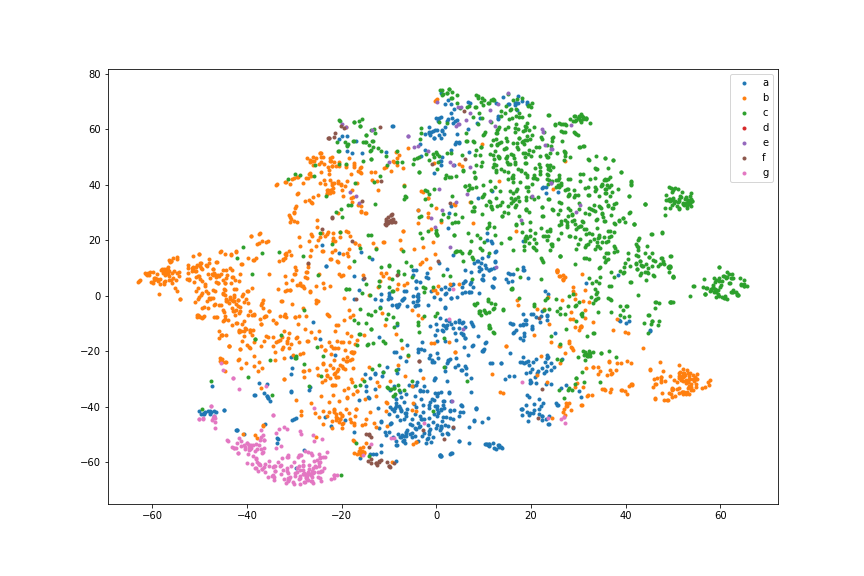
\includegraphics[width=0.4\linewidth]{latex/imgs/tsne_1_layer_with_schedule_512_final.png}
  	% Accuracy on test set: 13.03%, loss 2.83
  	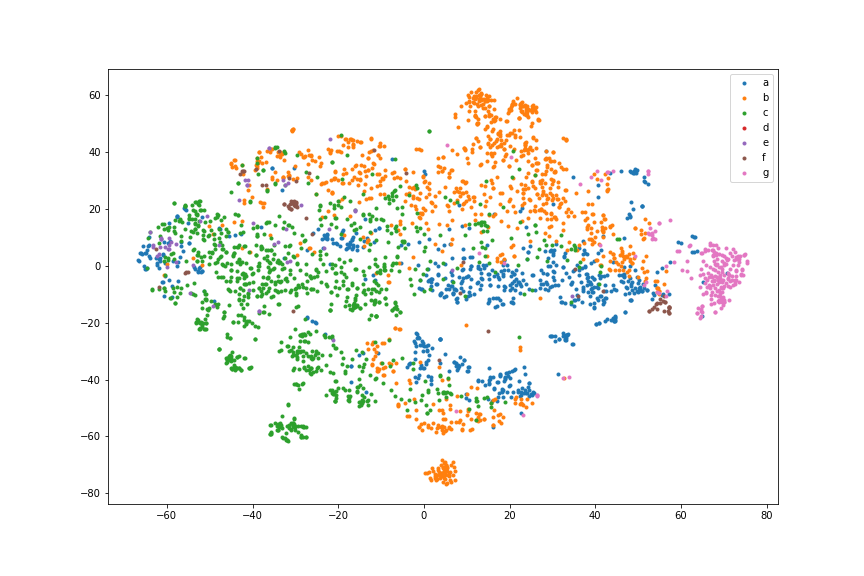
\includegraphics[width=0.4\linewidth]{latex/imgs/tsne_2_layer_no_drop_final.png}
	\caption{TSNE dimensionality reduction of the two models. Left is 1-layer, right is 2-layer}
\end{figure}

\begin{figure}[h]
	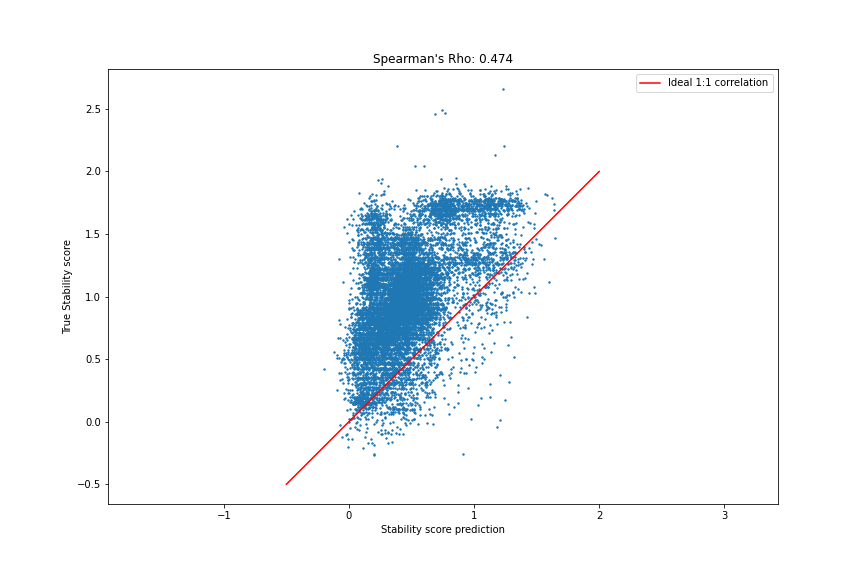
\includegraphics[width=0.4\linewidth]{latex/imgs/spearman_1_layer_with_schedule_512_final.png}
	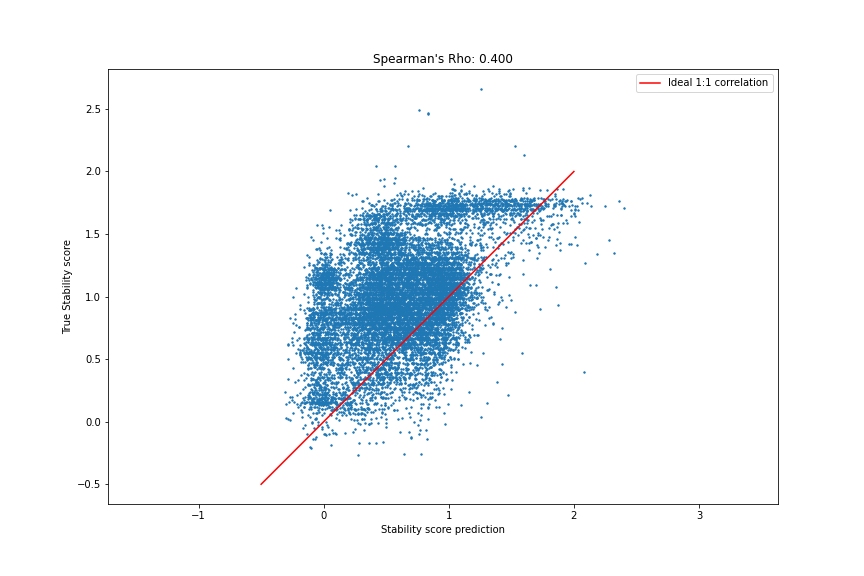
\includegraphics[width=0.4\linewidth]{latex/imgs/spearman_2_layer_no_drop_final.png}
	\caption{Plots used to calculate the Spearman correlation. Left is 1-layer, right is 2-layer}
\end{figure}

\begin{table}[]
\begin{tabular}{|l|l|l|l|}
\hline
        & Next token prediction accuracy & Test Loss & Spearman's rho\\ \hline
1-layer & 12.43\%                        & 2.84      & 0.400         \\ \hline
2-layer & 13.03\%                        & 2.83      & 0.428         \\ \hline
\end{tabular}
\end{table}

\subsubsection{Dropout vs. no dropout} % Finished
\begin{figure}[!ht]
  \centering
  % Accuracy on test set: 13.03%, loss 2.83
  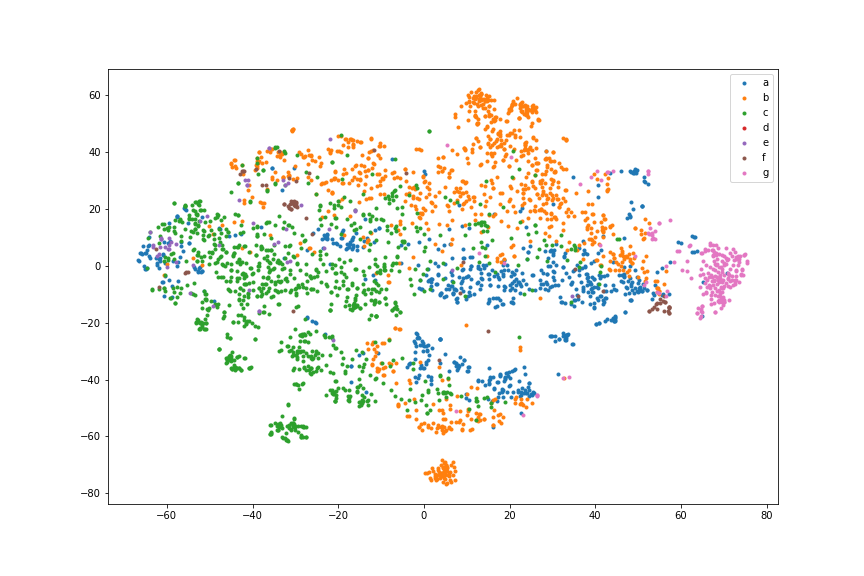
\includegraphics[width=0.49\linewidth]{latex/imgs/tsne_2_layer_no_drop_final.png}
  % Accuracy on test set: 13.02%, loss 2.82
  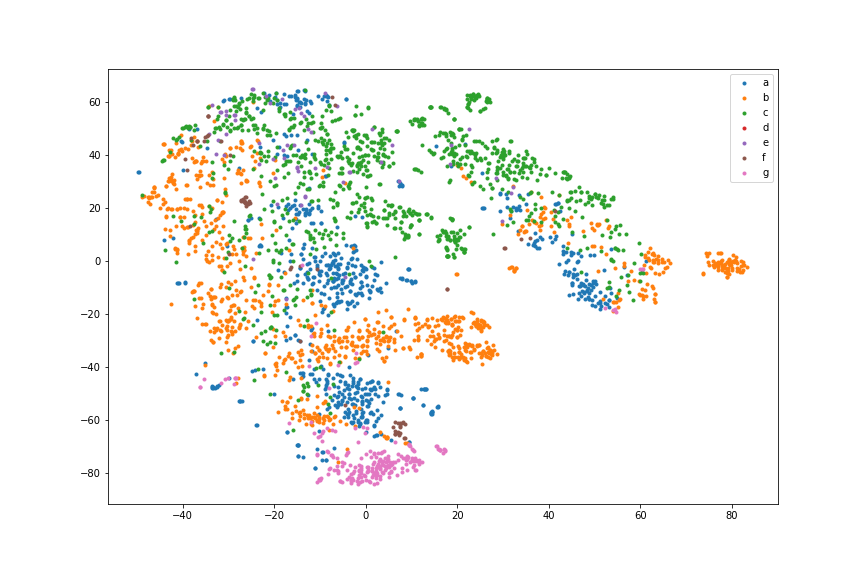
\includegraphics[width=0.49\linewidth]{latex/imgs/tsne_2_layer_05_drop_final.png}
  % 0.400 and 0.427
  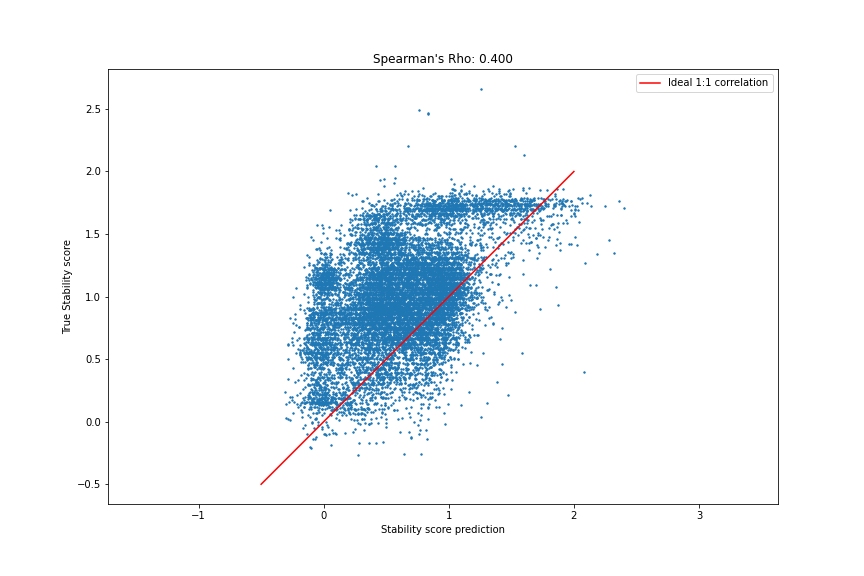
\includegraphics[width=0.49\linewidth]{latex/imgs/spearman_2_layer_no_drop_final.png}
  % 0.518 and 0.539
  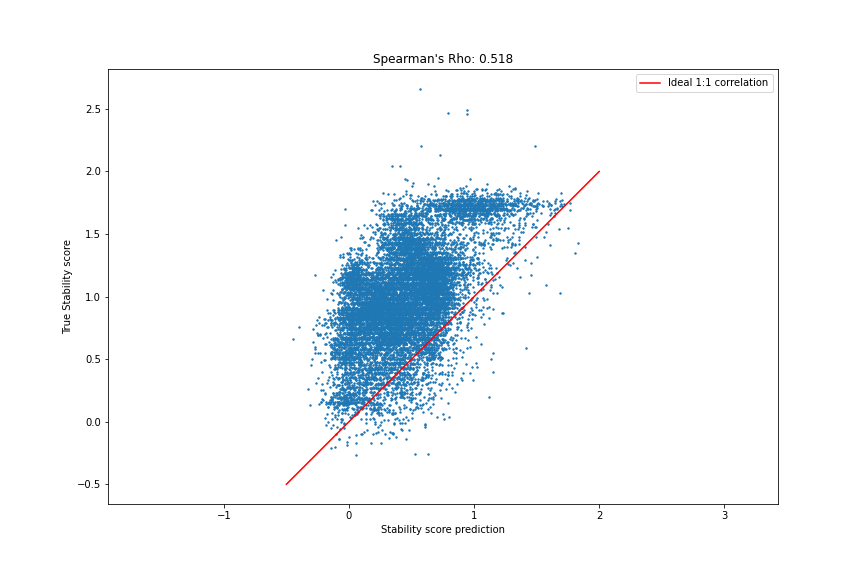
\includegraphics[width=0.49\linewidth]{latex/imgs/spearman_2_layer_05_drop_final.png}
  \caption{TSNE dimensionality reduction  and Spearman's rho data plots of the two models. Left is without dropout, right is with $50\%$ dropout.}
  \label{fig:cluster_spearman}
\end{figure}

\begin{table}[!ht]
\begin{tabular}{|l|l|l|l|}
\hline
             & Next token prediction accuracy & Test Loss & Spearman's rho\\ \hline
No dropout   & 13.03\%                        & 2.83      & 0.400         \\ \hline
50\% dropout & 13.02\%                        & 2.82      & 0.518         \\ \hline
\end{tabular}
\end{table}

\subsubsection{Feature size} % Finished
The feature size is the hyperparameter which controls the size of the internal layers of the LSTM. Increasing this should mean that the network can learn more complex functions. However, it also increases training time in a linear way. The increase is linear because for every feature you add, you have to backpropagate through one more. For this experiment we've trained three models with the following identical hyperparameters:
\begin{itemize}
	\item Layers: $1$
	\item Character embedding size: 30
	\item Starting learning rate: $8e-4$
	\item Learning rate schedule: Multiply by $0.2$ every 5 epochs
	\item Training time: 6 hours
\end{itemize}
The only difference between the models is the hidden layer size or feature size. We trained three models, one with $128$ features, one with $256$ features and one with $512$ features. Since training time is the most sparse resource for us, we decided that we would compare the results for equal real-time training time, not the number of epochs as with the other experiments.\\

\noindent
For this experiment we expect there to be some middle ground between the size of the model and how well it learns the representation. Since protein structures are very complex, we hypothesise that the larger models will perform better, even though they are not able to train for as many epochs.

\subsubsection{Learning rate} % Finished
\begin{figure}[!ht]
  \centering
  % Accuracy on test set: 13.34%, loss 2.83
  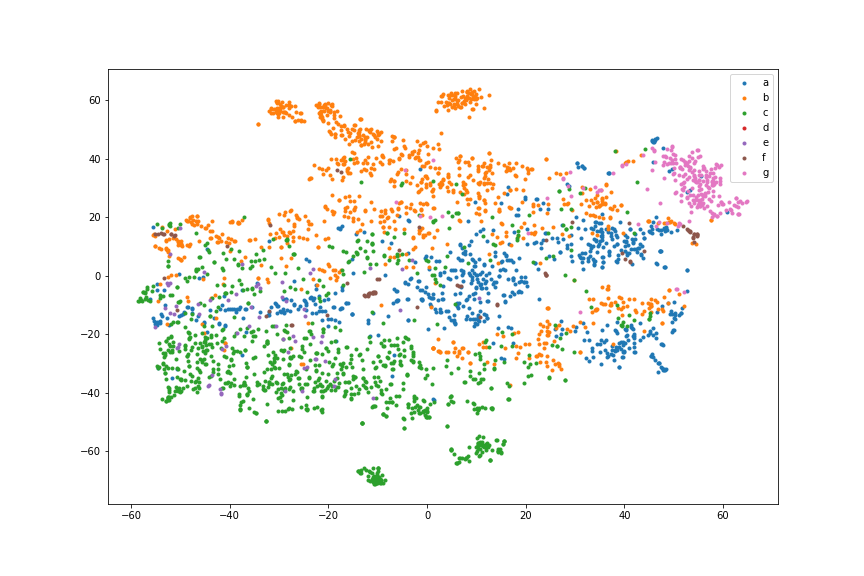
\includegraphics[width=0.49\linewidth]{latex/imgs/tsne_1_layer_no_schedule_512_final.png}
  % Accuracy on test set: 12.43%, loss 2.84
  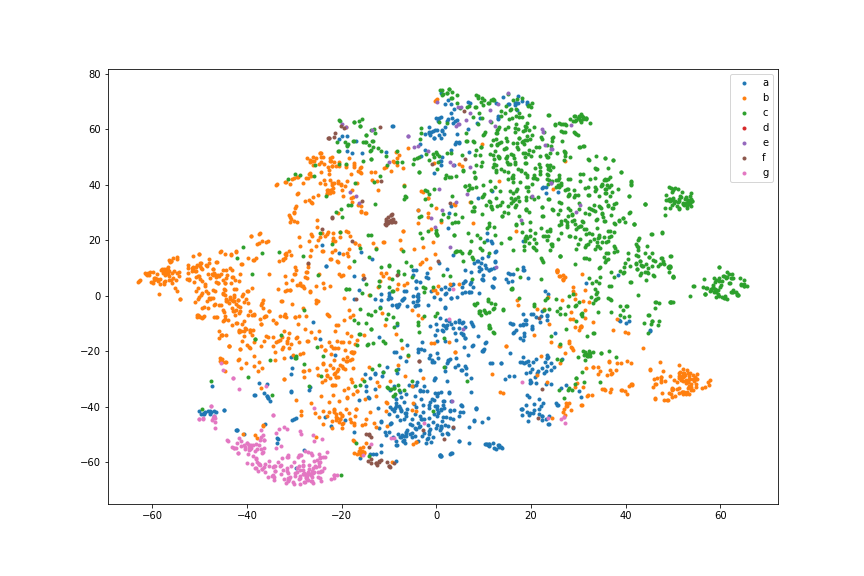
\includegraphics[width=0.49\linewidth]{latex/imgs/tsne_1_layer_with_schedule_512_final.png}
  % 0.605 and 0.592
  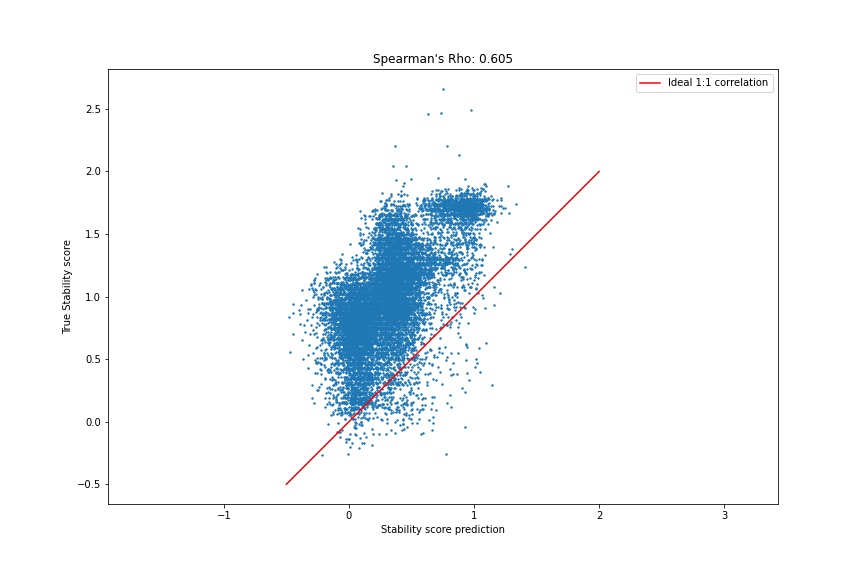
\includegraphics[width=0.49\linewidth]{latex/imgs/spearman_1_layer_no_schedule_512_final.png}
  % 0.428 and 0.414
  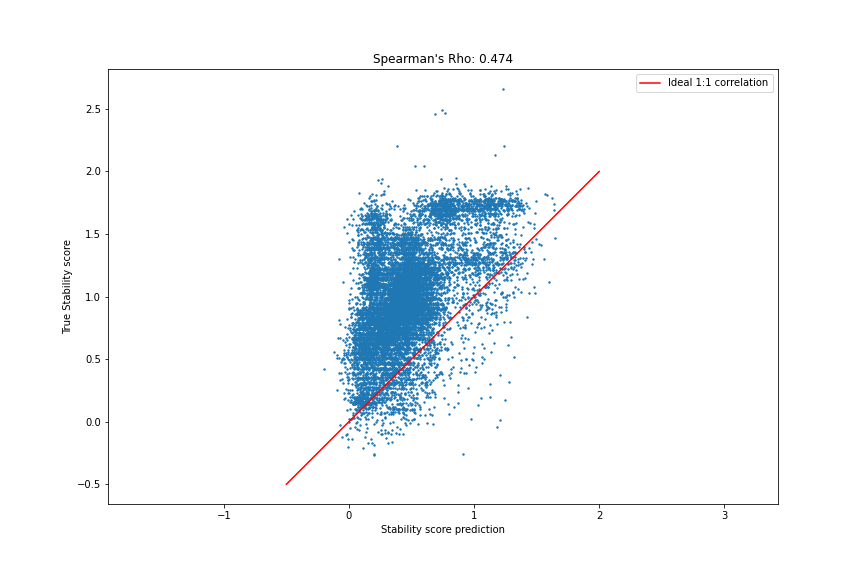
\includegraphics[width=0.49\linewidth]{latex/imgs/spearman_1_layer_with_schedule_512_final.png}
  \caption{TSNE dimensionality reduction  and Spearman's rho data plots of the two models. Left is without no learning rate schedule, right is with the schedule mention in the experiments section.}
\end{figure}

\begin{table}[!ht]
\begin{tabular}{|l|l|l|l|}
\hline
              & Next token prediction accuracy & Test Loss & Spearman's rho\\ \hline
No schedule   & 13.34\%                        & 2.83      & 0.605         \\ \hline
With schedule & 12.43\%                        & 2.84      & 0.474         \\ \hline
\end{tabular}
\end{table}

\subsubsection{Minimum loss model vs last model} % Finished
For this experiment we will not include the TSNE plots.
\begin{figure}[!ht]
  \centering
  % 0.518 and 0.539
  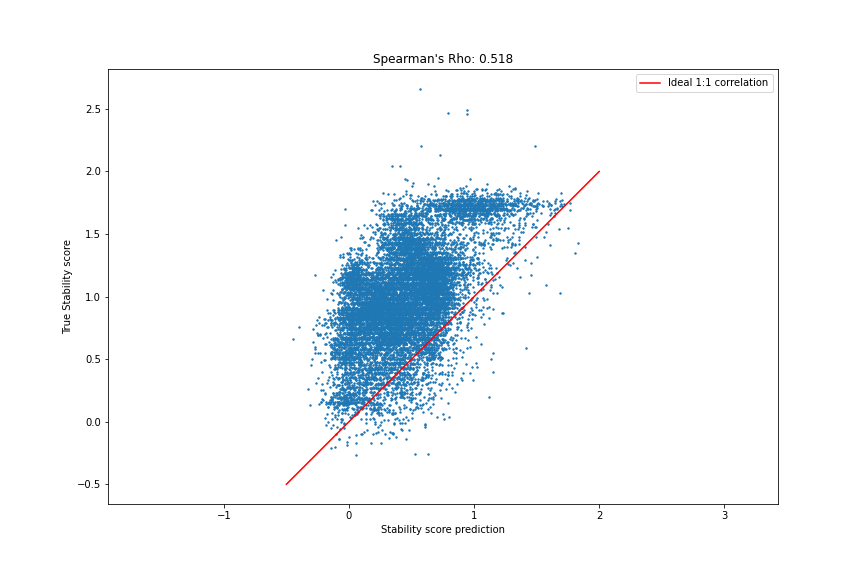
\includegraphics[width=0.49\linewidth]{latex/imgs/spearman_2_layer_05_drop_final.png}
  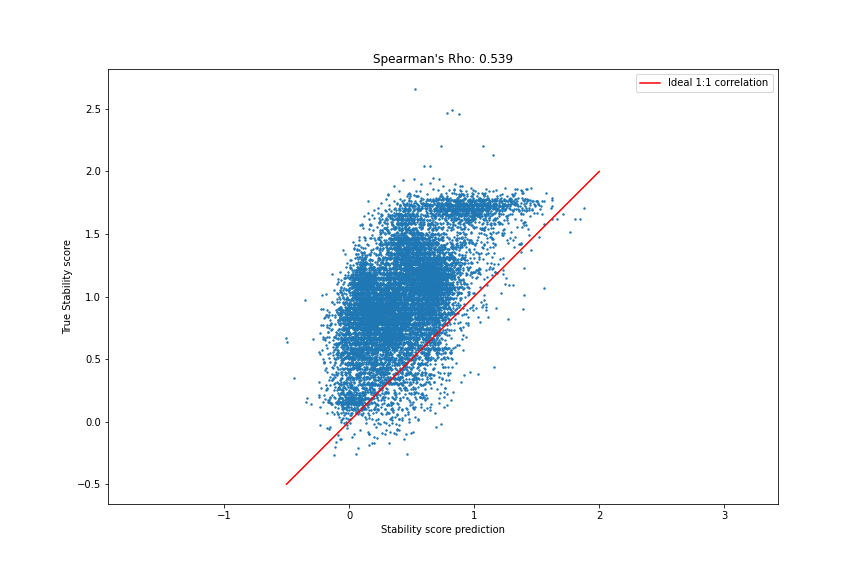
\includegraphics[width=0.49\linewidth]{latex/imgs/spearman_2_layer_05_drop_minloss.png}
  % 0.400 and 0.427
  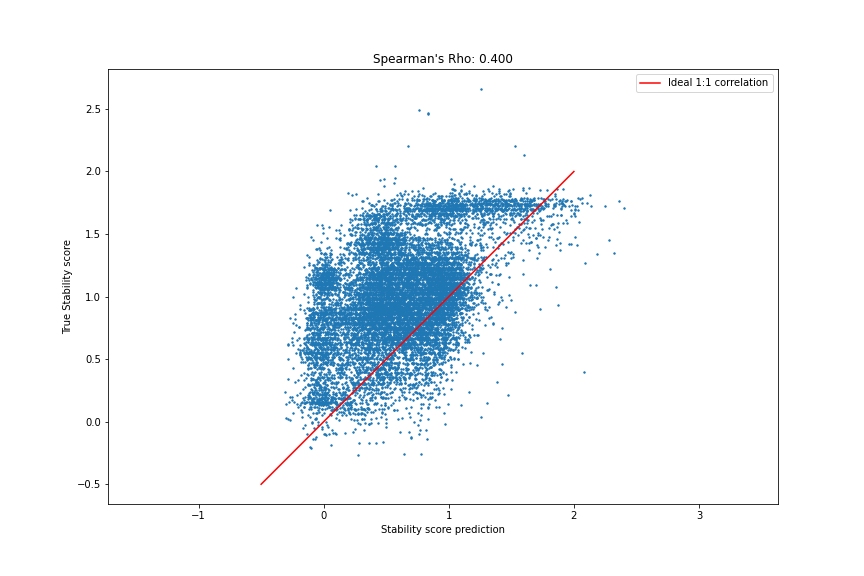
\includegraphics[width=0.49\linewidth]{latex/imgs/spearman_2_layer_no_drop_final.png}
  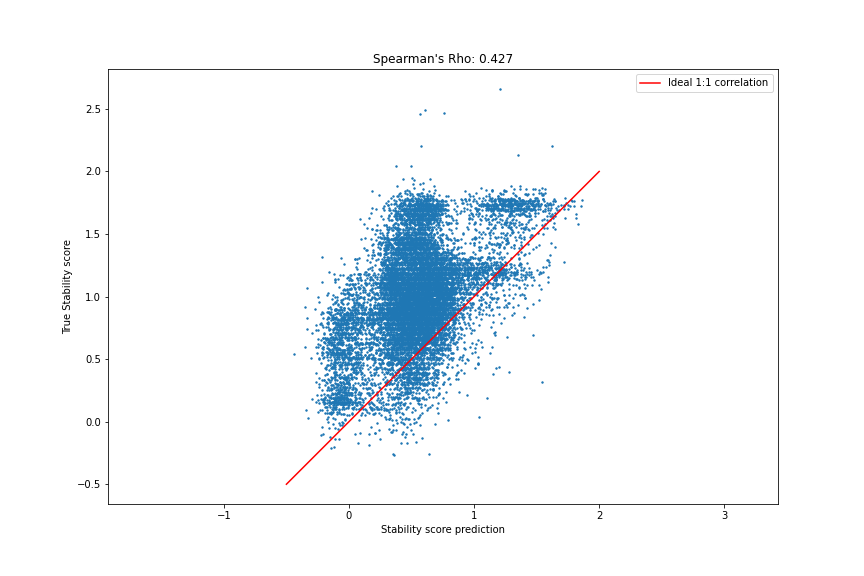
\includegraphics[width=0.49\linewidth]{latex/imgs/spearman_2_layer_no_drop_minloss.png}
  % 0.605 and 0.592
  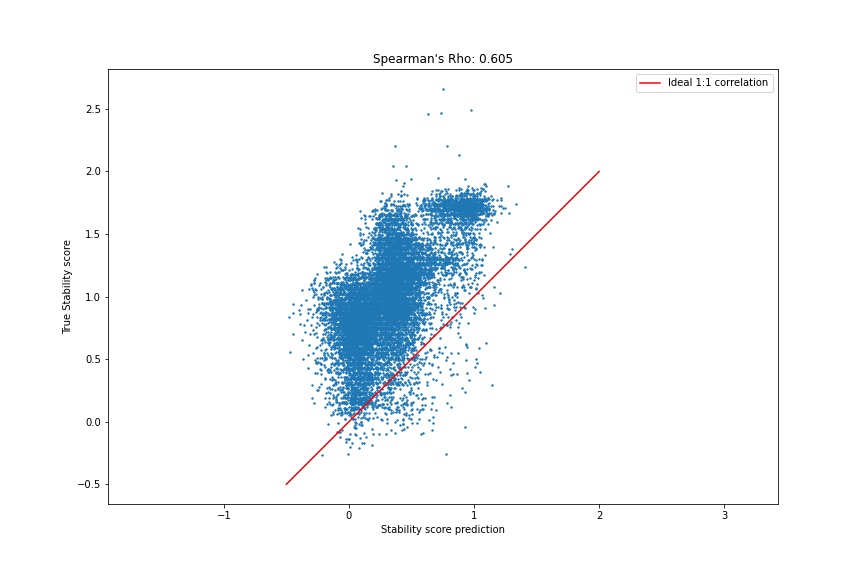
\includegraphics[width=0.49\linewidth]{latex/imgs/spearman_1_layer_no_schedule_512_final.png}
  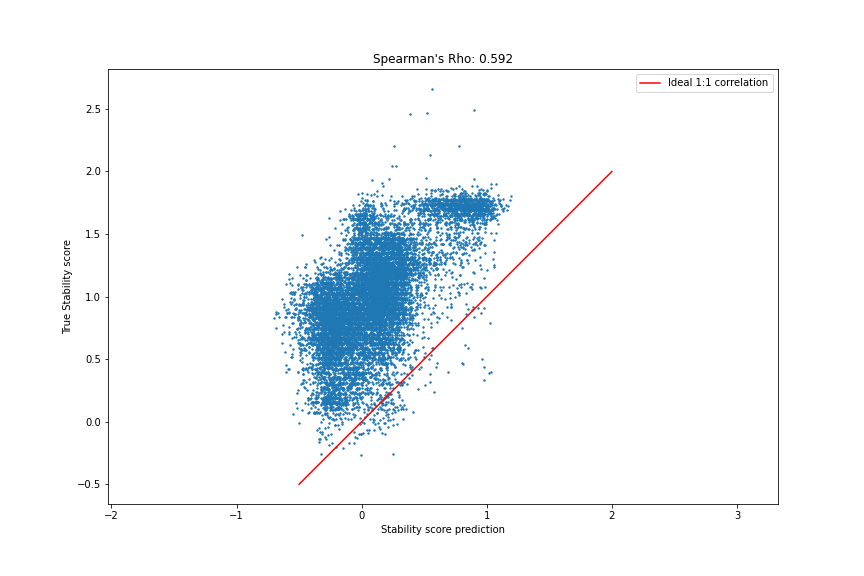
\includegraphics[width=0.49\linewidth]{latex/imgs/spearman_1_layer_no_schedule_512_minloss.png}
  % 0.428 and 0.414
  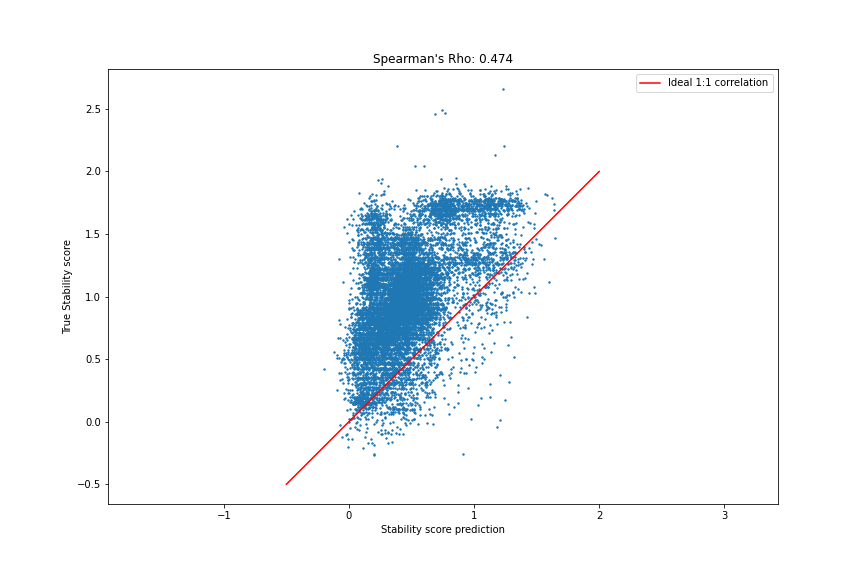
\includegraphics[width=0.49\linewidth]{latex/imgs/spearman_1_layer_with_schedule_512_final.png}
  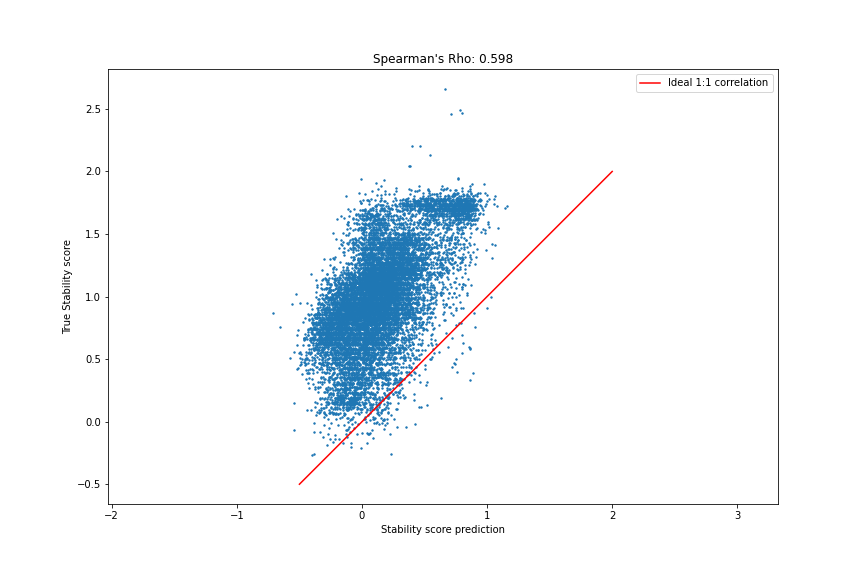
\includegraphics[width=0.49\linewidth]{latex/imgs/spearman_1_layer_with_schedule_512_minloss.png}
  % 0.435 and 0.424
  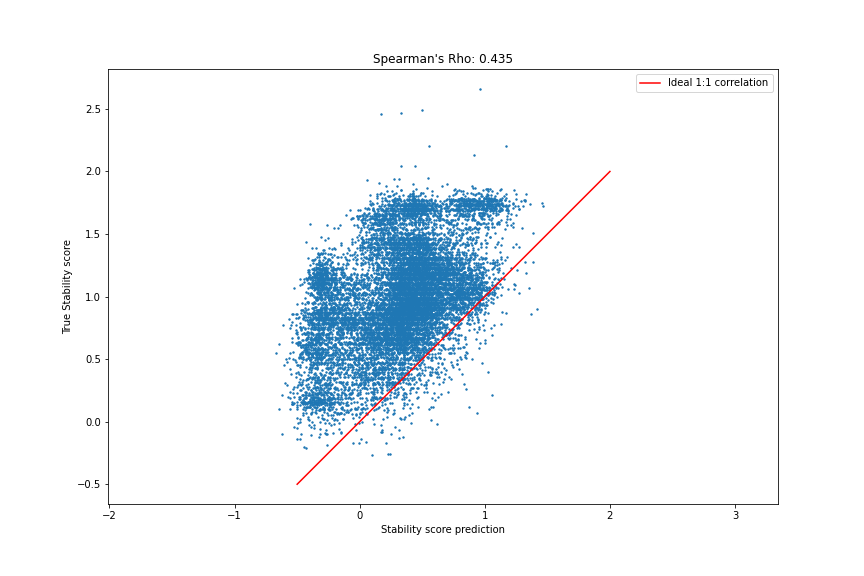
\includegraphics[width=0.49\linewidth]{latex/imgs/spearman_1_layer_with_schedule_256_final.png}
  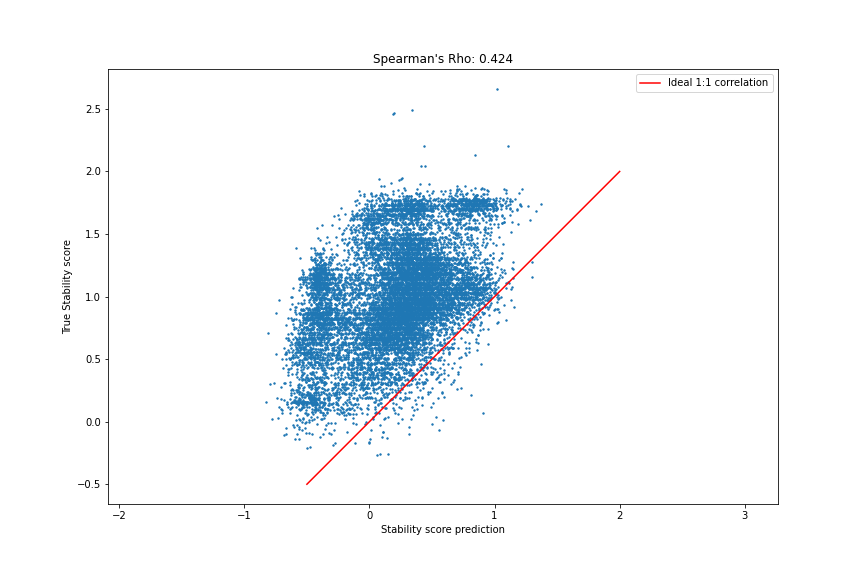
\includegraphics[width=0.49\linewidth]{latex/imgs/spearman_1_layer_with_schedule_256_minloss.png}
  % 0.507 and 0.627
  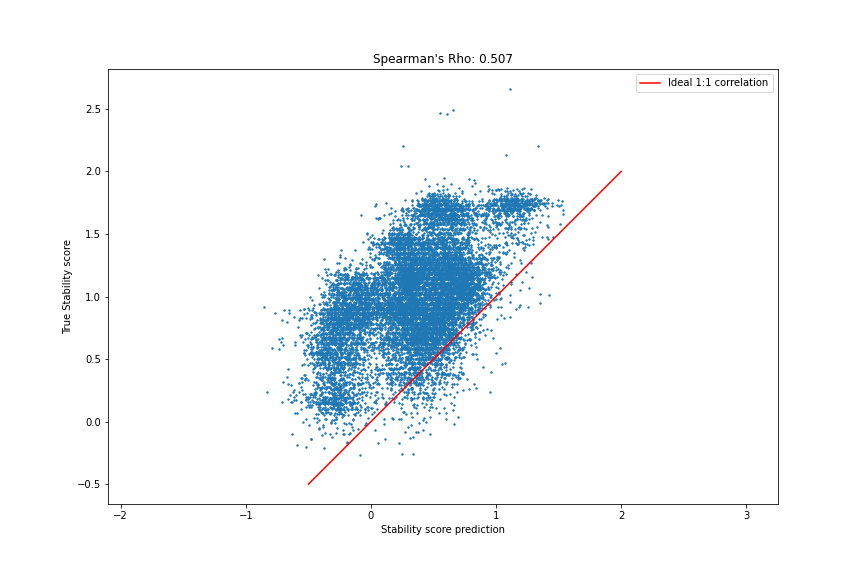
\includegraphics[width=0.49\linewidth]{latex/imgs/spearman_1_layer_with_schedule_1024_final.png}
  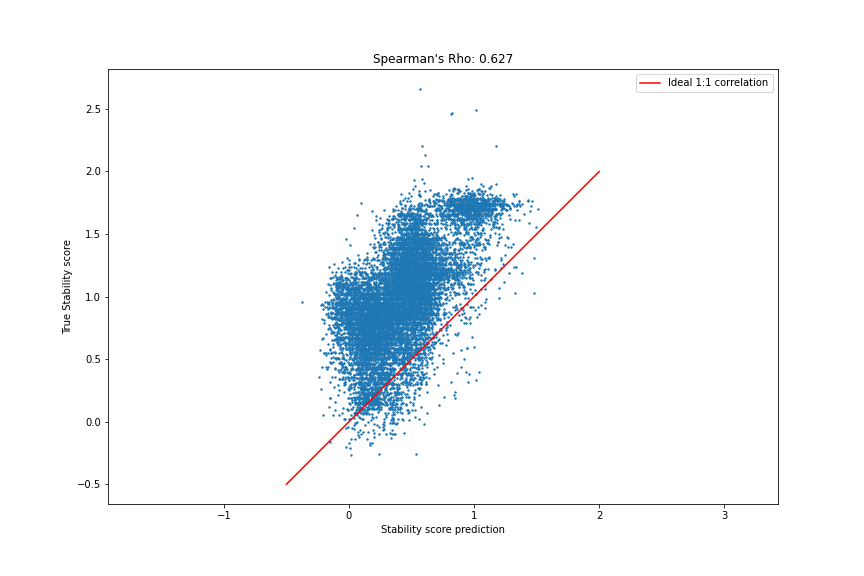
\includegraphics[width=0.49\linewidth]{latex/imgs/spearman_1_layer_with_schedule_1024_minloss.png}
  \caption{TSNE dimensionality reduction  and Spearman's rho data plots of the two models. Left is without no learning rate schedule, right is with the schedule mention in the experiments section.}
\end{figure}

\begin{table}[!ht]
\begin{tabular}{|l|lll|}
\hline
                                      &                                                     & Final Models                       &                \\ \cline{2-4} 
                                      & \multicolumn{1}{l|}{Next token prediction accuracy} & \multicolumn{1}{l|}{Test Loss}     & Spearman's rho \\ \hline
2-layer, 50\% dropout, 512 features   & \multicolumn{1}{l|}{13.02\%}                        & \multicolumn{1}{l|}{2.82}          & 0.518          \\ \hline
2-layer, no dropout, 512 features     & \multicolumn{1}{l|}{13.03\%}                        & \multicolumn{1}{l|}{2.83}          & 0.400          \\ \hline
1-layer, no lr schedule, 512 features & \multicolumn{1}{l|}{13.34\%}                        & \multicolumn{1}{l|}{2.83}          & \textbf{0.605} \\ \hline
1-layer, 256 features                 & \multicolumn{1}{l|}{11.41\%}                        & \multicolumn{1}{l|}{2.86}          & 0.435          \\ \hline
1-layer, 512 features                 & \multicolumn{1}{l|}{12.43\%}                        & \multicolumn{1}{l|}{2.84}          & 0.428          \\ \hline
1-layer, 1024 features                & \multicolumn{1}{l|}{\textbf{14.37\%}}               & \multicolumn{1}{l|}{\textbf{2.79}} & 0.507          \\ \hline
\end{tabular}
\end{table}
\begin{table}[!ht]
\begin{tabular}{|l|lll|}
\hline
                                      &                                                     & Minloss models                     &                \\ \cline{2-4} 
                                      & \multicolumn{1}{l|}{Next token prediction accuracy} & \multicolumn{1}{l|}{Test Loss}     & Spearman's rho \\ \hline
2-layer, 50\% dropout, 512 features   & \multicolumn{1}{l|}{13.03\%}                        & \multicolumn{1}{l|}{2.82}          & 0.539          \\ \hline
2-layer, no dropout, 512 features     & \multicolumn{1}{l|}{13.78\%}                        & \multicolumn{1}{l|}{2.81}          & 0.427          \\ \hline
1-layer, no lr schedule, 512 features & \multicolumn{1}{l|}{13.36\%}                        & \multicolumn{1}{l|}{2.83}          & 0.592          \\ \hline
1-layer, 256 features                 & \multicolumn{1}{l|}{11.40\%}                        & \multicolumn{1}{l|}{2.87}          & 0.424          \\ \hline
1-layer, 512 features                 & \multicolumn{1}{l|}{12.43\%}                        & \multicolumn{1}{l|}{2.85}          & 0.414          \\ \hline
1-layer, 1024 features                & \multicolumn{1}{l|}{\textbf{14.22\%}}               & \multicolumn{1}{l|}{\textbf{2.80}} & \textbf{0.627} \\ \hline
\end{tabular}
\end{table}

\subsection{CNN} % marc
\subsubsection{Latent representation} % marc
Using the CNN we reduce the dimension of each sequence to some latent representation $z$. Using $z$ in combination with t-sne, the goal was to get a two dimensional representation of each sequence, showing that some seperation could be seen in between the structures. \\

\noindent
During the experimenting with this model, we worked with a learning rate of $lr=1e-4$ and a batch size of 32. Since we experienced that introducing a too steep bottle neck would yield worse results, we decided to reduce the channel size down to 4 dimensions. \\

\noindent
The way our experiements vary from each other is how much we reduce the feature-dimension. Our two experiements work with the latent feature-dimensions 50 and 100. thus the $z$ will either have a size of $4$x$50$ or $4$x$100$. the latent representation will then get flattened and used in t-sne. \\

